%----------------------------------------------------------------------------------------
%	PACKAGES AND THEMES
%----------------------------------------------------------------------------------------

\documentclass{beamer}

\mode<presentation> {

% The Beamer class comes with a number of default slide themes
% which change the colors and layouts of slides. Below this is a list
% of all the themes, uncomment each in turn to see what they look like.

%\usetheme{default}
%\usetheme{AnnArbor}
%\usetheme{Antibes}
%\usetheme{Bergen}
%\usetheme{Berkeley}
%\usetheme{Berlin}
%\usetheme{Boadilla}
%\usetheme{CambridgeUS}
%\usetheme{Copenhagen}
%\usetheme{Darmstadt}
%\usetheme{Dresden}
%\usetheme{Frankfurt}
%\usetheme{Goettingen}
%\usetheme{Hannover}
%\usetheme{Ilmenau}
%\usetheme{JuanLesPins}
%\usetheme{Luebeck}
\usetheme{Madrid}
%\usetheme{Malmoe}
%\usetheme{Marburg}
%\usetheme{Montpellier}
%\usetheme{PaloAlto}
%\usetheme{Pittsburgh}
%\usetheme{Rochester}
%\usetheme{Singapore}
%\usetheme{Szeged}
%\usetheme{Warsaw}

% As well as themes, the Beamer class has a number of color themes
% for any slide theme. Uncomment each of these in turn to see how it
% changes the colors of your current slide theme.

%\usecolortheme{albatross}
%\usecolortheme{beaver}
%\usecolortheme{beetle}
%\usecolortheme{crane}
%\usecolortheme{dolphin}
%\usecolortheme{dove}
%\usecolortheme{fly}
%\usecolortheme{lily}
%\usecolortheme{orchid}
%\usecolortheme{rose}
%\usecolortheme{seagull}
%\usecolortheme{seahorse}
%\usecolortheme{whale}
%\usecolortheme{wolverine}

%\setbeamertemplate{footline} % To remove the footer line in all slides uncomment this line
%\setbeamertemplate{footline}[page number] % To replace the footer line in all slides with a simple slide count uncomment this line

%\setbeamertemplate{navigation symbols}{} % To remove the navigation symbols from the bottom of all slides uncomment this line
}

\usepackage{graphicx} % Allows including images
\usepackage{booktabs} % Allows the use of \toprule, \midrule and \bottomrule in tables
\usepackage{amsmath}
\usepackage{amssymb}
\newcommand{\rank}{\mathrm{rank}}

%----------------------------------------------------------------------------------------
%	TITLE PAGE
%----------------------------------------------------------------------------------------

\title[Direct Methods for GPs]{Summary of: Direct Methods for Gaussian Processes by O'Neil et. al.} % The short title appears at the bottom of every slide, the full title is only on the title page

\author{Jon Eskreis-Winkler} % Your name
\institute[UChicago] % Your institution as it will appear on the bottom of every slide, may be shorthand to save space
{
University of Chicago \\ % Your institution for the title page
\medskip
\textit{eskreiswinkler@uchicago.edu} % Your email address
}
\date{\today} % Date, can be changed to a custom date

\begin{document}

\begin{frame}
\titlepage % Print the title page as the first slide
\end{frame}

\begin{frame}
\frametitle{Overview} % Table of contents slide, comment this block out to remove it
\tableofcontents % Throughout your presentation, if you choose to use \section{} and \subsection{} commands, these will automatically be printed on this slide as an overview of your presentation
\end{frame}

%----------------------------------------------------------------------------------------
%	PRESENTATION SLIDES
%----------------------------------------------------------------------------------------

%------------------------------------------------
\section{What is a Gaussian Process?}% Sections can be created in order to organize your presentation into discrete blocks, all sections and subsections are automatically printed in the table of contents as an overview of the talk
%------------------------------------------------

% A subsection can be created just before a set of slides with a common theme to further break down your presentation into chunks

\begin{frame}
\frametitle{Gaussian Process motivation and definition}

\begin{itemize}
\item Given data $(\textbf{X}_n, \textbf{Y}_n)=(X_1, Y_1), \dots, (X_n, Y_n)$, how do you infer what type of process generated the data and responses? -- enable predictions for future data.
\item Frequentists just use regression; alternative approach is probabilistic...
\item The posterior probability distribution for the process $f: \mathcal{X}^n \rightarrow \mathcal{Y}^n$ is 
$$P(f|\textbf{X}_n, \textbf{Y}_n) = \frac{P(\textbf{Y}_n|f, \textbf{X}_n)P(f)}{P(\textbf{Y}_n|\textbf{X}_n)}$$
\item What is the function space to which $f$ belongs? Need to restrict the space if we want to be able to measure the numerator terms.
\item Simplifying assumption: $f$ is a Gaussian Process.
\item A mapping $f$ is called a \textbf{Gaussian Process} if for any $m\in\mathbb{N}$, for any $m$-length  input set $(X_1, \dots, X_m)$, the distribution of $(f(X_1), \dots, f(X_m))$ is multivariate normal.
\end{itemize}
\end{frame}

%------------------------------------------------

\begin{frame}
\frametitle{Gaussian Process Intuition}
\begin{itemize}
\item Gaussian Process generalizes the notion of a finite dimensional Gaussian distribution to an infinite dimensional analog
$$X \sim \mathcal{N}(\mu, \Sigma) \Longleftrightarrow f(\textbf{X}_n) \sim \mathcal{N}(\mu(\textbf{X}_n), \Sigma(\textbf{X}_n))$$
The mean and covariance functions are defined by the data.

\item $\Sigma(\textbf{X}_n)_{ij} = K(\textbf{X}_n)_{ij} = k(x_i,x_j)$ for some kernel $k$ where $k$ is a positive semidefinite kernel, meaning that $K$ is a PSD kernel matrix.
\item We will see that, for prediction, the covariance function $\Sigma_p(\textbf{X}_n)$ is often of the form $\Sigma(\textbf{X}_n) = \sigma^2 I + K$.
\end{itemize}
\end{frame}

\begin{frame}
\begin{itemize}
\item We can now define the prior on $f$, $P(f)$, using this formalism. Assuming for simplicity that $\mu(x) = 0$, the prior for $f$ is the density for an $n$-dimensional multivariate normal:
$$P(f(\textbf{X}_n)) = (2\pi)^{-\frac{n}{2}} \det( \Sigma(\textbf{X}_n))^{-\frac{1}{2}} \exp \left(-\frac{1}{2} f(\textbf{X}_n)\Sigma(\textbf{X}_n)^{-1} f(\textbf{X}_n) \right)$$
\item To make predictions, we consider the distribution for $\textbf{Y}_n | \textbf{X}_n$
$$Y_{n+1} | \textbf{X}_n, \textbf{Y}_n, X_{n+1} \sim N(\tilde{\mu}(x), \tilde{\Sigma}(x))$$
where $\tilde{\mu}, \tilde{\Sigma}$ are functions of the data. The resulting likelihood function involves inverting a matrix of the form $(\sigma^2 I + \Sigma(\textbf{X}_n))^{-1}$.

\end{itemize}
\end{frame}

%------------------------------------------------
\subsection{Computational Bottleneck} 
\begin{frame}
\frametitle{Computational Bottleneck}
\begin{block}{Common computational complexities}
\begin{itemize}
\item Using Gauss-Jordan elimination, matrix inversion has complexity $O(n^3)$.
\item Finding determinant of a matrix by LU decomposition has complexity $O(n^3)$.
\end{itemize}
\end{block}
\begin{itemize}
\item For large $n$, this makes computation of posterior distributions for Gaussian Processes intractable -- recall the inverse and determinant in the likelihood function.
\item What can be done?
\end{itemize}

\end{frame}

%------------------------------------------------
\section{Options for "Accelerated" Methods: Direct and Indirect}
\begin{frame}
\frametitle{Accelerated Methods for inversion/determinant of matrix of form $C=I+K$}

\textbf{Types}

\begin{enumerate}
\item Direct Methods
	\begin{itemize}
		\item $rank(K) = p <<n \Rightarrow$ use Sherman-Morrison-Woodbury 		formula and Sylvester det. theorem in $O(p^2 n)$ each. It is typically not 		easy to identify if $K$ is low rank, or if it is approximately low rank.
	\end{itemize}
\item Iterative Methods
	\begin{itemize}
		\item Fast Gauss Transform and Fast Fourier Transform: can speed up matrix multiplication to help with determinant but inverse will still be hard?
	\end{itemize}
\end{enumerate}

Broad distinction between two main approaches: low rank approximations that assume $K$ is a finite rank operator (will be a dense entry-wise but "data-sparse") vs. thresholding actual entries of the matrix (matrix will be sparse, but has high numerical rank).

The paper's method makes an approximation at the "level of the covariance matrix."
\end{frame}



%------------------------------------------------
\section{Suggested Approach for HODLR Matrices}
\subsection{What is a HODLR matrix?}
\begin{frame}
\frametitle{HODLR Matrix definition}
Hierarchical Off-Diagonal Low-Rank Matrices (\textbf{HODLR}) are a class of matrices that have off-diagonal blocks that are easily represented recursively, each of which have low rank (we focus on symmetric matrices).
\begin{center}
 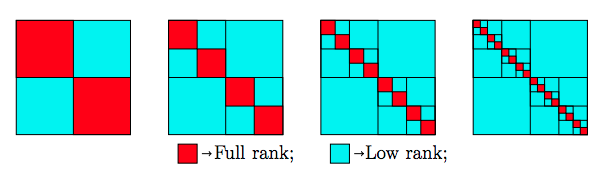
\includegraphics[width=0.5\textwidth]{fig1.png}\end{center}
 \end{frame}
 
 \begin{frame}
 \frametitle{HODLR examples}
 Example:  For $K_0 \in \mathbb{S}^n$, $K_0$ is a two level HODLR matrix if
 $$K_0 = \begin{pmatrix} K_1^{(1)} & U_1^{(1)}V_1^{(1)^T} \\ V_1^{(1)}U_1^{(1)^T} & K_2^{(1)}\\ \end{pmatrix}, \ U_1^{(1)}, V_1^{(1)} \in \mathbb{R}^{\frac{n}{2}\times r}, \ r << n$$
 $$K_1^{(1)} = \begin{pmatrix} K_{1,1}^{(2)} & U_1^{(2)} V_1^{(2)^T} \\ V_1^{(2)} U_1^{(2)^T} & K_{1,2}^{(2)} \\ \end{pmatrix}, K_2^{(1)} = \begin{pmatrix} K_{2,1}^{(2)} & U_2^{(2)} V_2^{(2)^T} \\ V_2^{(2)} U_2^{(2)^T} & K_{2,2}^{(2)} \\ \end{pmatrix}$$ 
$$U_i^{(2)}, V_i^{(2)} \in \mathbb{R}^{\frac{n}{4}\times r}, \ \forall (i,j) \in \{1,2\}^2, \ K_{i,j}^{(2)} \in \mathbb{R}^{\frac{n}{4}\times \frac{n}{4}}$$
\end{frame}

\begin{frame}
\frametitle{A suggested factorization for HODLR matrices}
Without explaining how it will be obtained, suppose that we are given a factorization of $K = \prod_{i=0}^\kappa K_i$. \\
For $\kappa=2$, $K = K_2 K_1 K_0 \Leftrightarrow$:
\begin{center}
 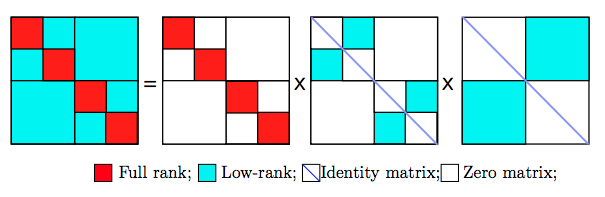
\includegraphics[width=0.5\textwidth]{fig2.png}\end{center}
For $\kappa=3$, $K =K_3 K_2 K_1 K_0 \Leftrightarrow$:
\begin{center}
 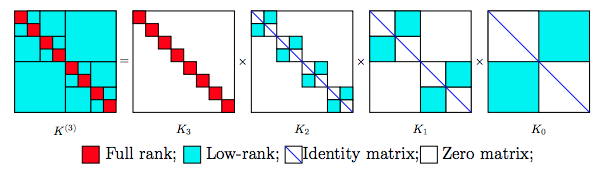
\includegraphics[width=0.5\textwidth]{fig3.png}\end{center}
 \end{frame}
 \subsection{Matrix Inversion}
 \begin{frame}
 \frametitle{Why is this helpful? Matrix Inversion!}
 \begin{itemize}
 \item Consider $K = \begin{pmatrix} A & UV^T \\ VU^T & B \\ \end{pmatrix} = \begin{pmatrix} A & 0 \\ 0 & B \\ \end{pmatrix}+ \begin{pmatrix} 0 & UV^T \\ VU^T & 0 \\ \end{pmatrix} = \begin{pmatrix} A & 0 \\ 0 & B \\ \end{pmatrix}+ \begin{pmatrix} U & 0 \\ 0 & V \\ \end{pmatrix}\begin{pmatrix} 0 & V^T \\ U^T & 0 \\ \end{pmatrix}$
 \item Since $U,V$ are low rank, the matrix can be more easily inverted using the Sherman-Morrison-Woodbury Formula:
 $$(A+BC)^{-1} = A^{-1} - A^{-1}B(I+CA^{-1}B)^{-1}CA^{-1}$$
 $$\Leftrightarrow (I+BC)^{-1} = I-B(I+CB)^{-1}C$$
 Because of $B,C$ having very few columns, the middle term can be inverted very quickly. 
 \item To invert entire matrix, we can perform this procedure on each of the block of each component in $K = K_\kappa K_{\kappa-1} \cdots K_2 K_1 K_0$. We will usually have $\kappa \approx \log n$ so inversion can be computed in $\mathcal{O}(n\log n)$ because S-M-W formula inverse in $\mathcal{O}(n)$.
 \end{itemize}
 \end{frame}
  \subsection{Computing Determinant}
 \begin{frame}\frametitle{Why is this helpful? Computing Determinant!}
 \begin{block}{Sylvester's Determinant Theorem}
 For $A\in \mathbb{R}^{m\times n}, \ B \in \mathbb{R}^{n\times m},\ \det(I_m + AB) = \det(I_n+BA)$.
 \end{block}
 \begin{itemize}
 \item $K = \prod^\kappa_{i=0} K_i \Rightarrow \det K = \prod^\kappa_{i=0}  \det K_i$. $\det K_\kappa = \prod_{i=1}^{2^\kappa} \det K_{\kappa,i}$. For $k\neq \kappa$, $\det K_k$ is a low rank perturbation to the identity matrix, and we can use Sylvester's theorem on each diagonal block $j \in [1,2^{k+1}]$:
 $$\det\left(I_{\frac{n}{2^{k}}}+ \begin{pmatrix} U_j^{(k)} & 0 \\ 0 & V_j^{(k)} \\ \end{pmatrix}\begin{pmatrix} 0 & V_j^{(k)^T} \\ U_j^{(k)^T} & 0 \\ \end{pmatrix} \right)$$
 $$ = \det \left(I_{2r} +\begin{pmatrix} 0 &V_j^{(k)^T}V_j^{(k)}\\ U_j^{(k)^T}U_j^{(k)} & 0\\  \end{pmatrix} \right)$$
 \item Each matrix's computational cost using the theorem is $\mathcal{O}(n)$, so doing so for all $\kappa$ matrices costs $\mathcal{O}(n\log n)$.
 \end{itemize}
\end{frame}



\subsection{Algorithm for computing the factorization}
\begin{frame}
\frametitle{Algorithm for computing the factorization}
\begin{itemize}
\item Given a HODLR matrix $K\in \mathbb{R}^{n\times n}, \ K = \begin{pmatrix} A_{11} & A_{12} \\ A_{12}^T & A_{22}\\ \end{pmatrix}$ where $A_{11},A_{22}$ are full rank and $A_{12}=UV^T$ is low rank. The key is to note that:
$$K = \begin{pmatrix} A_{11} & UV^T \\ VU^T & A_22\\ \end{pmatrix} = \begin{pmatrix} A_{11} & 0 \\ 0 & A_{22}\\ \end{pmatrix}\begin{pmatrix} I_\frac{n}{2} & A_{11}^{-1}UV^T \\ A_{22}^{-1}VU^T & I_\frac{n}{2} \\ \end{pmatrix}$$
This might seem like an expensive algorithm, because $A_{11}$ might be large, but we do it recursively, and so only invert matrices that are $\kappa\times\kappa$.
\end{itemize}
\end{frame}
%------------------------------------------------
\subsection{Numerical Results}
\begin{frame}
\frametitle{Numerical Results in Computation}
\begin{itemize}
\item Experimented with matrix inversion and determinant computation for different covariance matrices $C=\sigma^2 I+K$ where $K$ is a PSD kernel matrix. Tested with kernel functions: (1) Gaussian covariance, (2) multiquadric covariance, (3) exponential covariance, (4) Inverse multiquadric and biharmonic kernels.
\item   Results are extremely impressive. They are tables II-V in O'Neil's paper.
\item When the dimension of the points was increased, the computation time explodes, and the meaningfulness of the spatial structure is compromised due to curse of dimensionality. Not an interesting application of this method at this time...
\item In a regression experiment, the RMSE of the regression line is inversely related to the factorization precision.
\end{itemize}
\end{frame}

\section{Conclusions}

\begin{frame}
\frametitle{Conclusions}
\begin{itemize}
\item Many covariance matrices used in GPs have the HODLR property, justifying the use of this method in many applications.
\item Future research needed to identify how to deal with cases when dimensionality of data is large.
\item No comparison is given to other methods' computation time and accuracy.
\item How does this compare to a more general multiscale method like MMF -- we may want to deal with structures other than HODLR.
\item Next step: compare computational results of MMF factorized matrices with this method on HODLR matrices.

\end{itemize}
\end{frame}




\end{document} 